\begin{figure} [h]
   \centering
   \psfrag{user}{\textcolor{blue}{\Large{user interaction}}}
   \psfrag{compute}{\textcolor{blue}{\Large{compute}}}
   \psfrag{storage}{\textcolor{blue}{\Large{store} (data base)}}
   \psfrag{ongoing}{(ongoing)}
   %
   \psfrag{Start}{\bf Start}
   \psfrag{Input}{input data}
   \psfrag{pdb}{PDB}
   \psfrag{exist}{existing atlas}
   \psfrag{initiate}{}
   %
   \psfrag{Propose}{{\bf Propose}}
   \psfrag{Intervene}{{\bf Intervene}}
   \psfrag{Redirect}{(re)direct}
   \psfrag{Refine}{refine}
   \psfrag{Limit}{limit}
   \psfrag{Complete}{complete}
   \psfrag{Stop}{stop}
   %
   \psfrag{View}{{\bf Query/View}}
   \psfrag{Query}{}
   %\psfrag{Query}{{\bf Query/View}}
   \psfrag{Atlas}{\footnotesize atlas view}
   \psfrag{all}{all}
   \psfrag{select node}{select node}
   \psfrag{Parameter}{Parameter View}
   \psfrag{boundaries}{boundaries}
   \psfrag{select parameter}{select configuration}
   \psfrag{Realization}{realization view}
   \psfrag{walkthrough}{walk through}
   %
   \psfrag{Combinatorial Graph}{ configuration \figref{fig:dumbelldialog}}
   \psfrag{Sample}{{\bf Sampling}}
   \psfrag{Algo}{Algorithm}
   \psfrag{ref}{\mred{\secref{sec:algorithms}}}  %sec:algor
   %\psfrag{ref2}{\mred{\secref{sec:realize}}}
   \psfrag{ref3}{\mred{\secref{sec:gui}}}   %sec:user
   \psfrag{ref4}{\mred{\secref{sec:intro}}}
   \psfrag{Navigate}{navigation}
   \psfrag{Realize}{{\bf realization}}
   \psfrag{Collision}{collision test}
   %
   \psfrag{DB}{{\Large{\bf  Atlas}}}
   \psfrag{sgraph}{\sgraph}
   \psfrag{reglab}{region labels (\cgraph s)}
   \psfrag{Parameter}{\footnotesize \shortstack[l]{Cayley \\ configurations}}
   \psfrag{Realization}{\footnotesize \shortstack[l]{Cartesian\\ realizations}}
\includegraphics[width=1.\textwidth] {fig/completefigure.eps}   
%\epsfig{file=\fig/completefigure.eps,width=1.\textwidth}
   \caption{ \EASAL\ overview that shows relations between different structures.}
   \label{fig:EASALLayout}
\end{figure}

%

%\section{EASAL Layout}
%\label{sec:user}

